% 英文で執筆する場合はクラスファイルへのオプションを[T,E]としてください.
% If you want to write your paper in English, pass to [T,E] options to document class.
\documentclass[T,J]{fose} % 「コンピュータソフトウェア」用のクラスファイルは compsoft です.
\taikai{2023} % 固定です.出版委員長が毎年変更してAuthor Kitを配布してください.

\usepackage [dvipdfmx] {graphicx}

% ユーザが定義したマクロなどはここに置く.ただし学会誌のスタイルの
% 再定義は原則として避けること.

% 以下は説明のために使用したパッケージであるため,削除可能.
\usepackage{fancyvrb}
\usepackage{url}
\usepackage{cite}
\usepackage{color}
\usepackage{graphicx}
\usepackage{multirow}
\usepackage{amsmath}
% \usepackage{threeparttable} 上手いこと使えない
% \usepackage[dvipdfmx]{color} クラッシュしていてなくても動くのでコメントアウト


\newcommand{\todo}[1]{\colorbox{yellow}{{\bf TODO}:}{\color{red} {\textbf{[#1]}}}}
\newcommand{\wrote}[1]{\colorbox{green}{{\bf Wrote}:} {\textbf{[#1]}}}
\newcommand{\checked}[3]{\colorbox{red}{ここまでチェック済み}}

\begin{document}

% 論文のタイトル
\title{複数プロジェクト開発履歴を用いた修正を要する\\規約違反ソースコード予測の試み}
% 以下の \etitle(と\@etitle)はFOSE論文フォーマット独自のマクロです.
% FOSEに投稿した論文を発展させてコンピュータソフトウェアに投稿される場合はコメントアウトしてください.
% \setetitleは奇数ページのヘッダに表示する文字列(\etitle)を設定するためのマクロです.
% タイトルが2行に渡る場合は "\\" を 使用することで任意の位置で改行をすることができます.
\setetitle{Toward Predicting Coding Violations Fixing using Multiple Project Dataset}
%\setetitle{Long Long Long Long Long Long \\ Long Long Long Long Long \\ Long Long Long Long Long Long Long Long Long Long Long Long Paper Title}

% タイトル,著者などが複数行にわたり,論文冒頭の著者名が日本語アブストと重複して描画された場合に以下のコメントアウトを外してください.
\longtitle

% 著者
% 和文論文の場合,姓と名の間には半角スペースを入れ,
% 複数の著者の間は全角スペースで区切る
%
\author{亀岡 令 伊原 彰紀 大森 楓己
%
% ここにタイトル英訳 (英文の場合は和訳) を書く.
% 英語タイトルは論文1ページ目左下,著者らの名前・所属一覧の一番上に表示される
%
% 上記\setetitle中で改行した場合は "\etitle" を削除し,改行(\\)を入れていないタイトルを記載してください.
% \ejtitleは1ページ目左下に挿入されるタイトルとして使用されます.
% また,"\etitle"はFOSE論文フォーマット独自のマクロです.
\ejtitle{\etitle}
%
% ここに著者英文表記 および
% 所属 (和文および英文) を書く.
% 複数著者の所属はまとめてよい.
%
% 複数著者の所属は以下のようにまとめてよい.
\shozoku{Ryo Kameoka, Akinori Ihara, Fuki Omori}{和歌山大学}
{Wakayama University}
}

%
% 和文アブストラクト
% In English paper, content of Jabstract will be ignored. 
\Jabstract{%
複数の開発者が参画するソフトウェア開発では.開発者は可読性,保守性の向上のために静的解析ツールを用いてコーディング規約に違反しているソースコードを検出し,修正に取り組む.しかし,静的解析ツールは規約違反の指摘漏れを抑えるため,大量の規約違反を出力し,その大半が開発者に修正されていない.従来研究では,規約違反を検証するプロジェクトの過去の修正履歴を学習したモデルを構築し,静的解析ツールの検出結果の中で優先的に修正すべき規約違反ソースコードを予測する手法を提案している.本研究では,従来研究において単一プロジェクトの学習によって十分に学習できない規約違反を,複数プロジェクトのデータの学習する予測モデルを構築し,当該モデルが多様な規約違反を予測可能か否かを明らかにする.10件のOSSプロジェクトを対象に実験を行った結果,学習データセットの小さいプロジェクト,正例データの少ないプロジェクトに対して本手法が有効であることを確認した.
}
%
% 英文アブストラクト(本サンプルの原論文にはなし)
% \Eabstract{
% }
%
\maketitle \thispagestyle {empty}
%%%%%%%%%%%%%%%%%%%%%%%%%%%%%%%%%%%%%%
\section{はじめに}
%%%%%%%%%%%%%%%%%%%%%%%%%%%%%%%%%%%%%%

複数人で実装するソフトウェア開発では,開発者間のコーディングスタイルを共通化することにより,ソースコードの可読性を高め,ソフトウェア保守が容易になることが知られている\cite{EffectsSAT}.コーディングスタイルを共通化するため,各プログラミング言語ではソースコードを記述するためのガイドラインとしてコーディング規約を公開している.具体的には,Java言語のJavaコーディング標準,Python言語のPEP8などがある.これらコーディング規約には命名規則やコメント文などに関するルールが定められている.

従来研究では,コーディング規約の導入により,ソフトウェア開発プロジェクトにとってソースコード理解の促進,バグの早期発見などに効果があることを明らかにしている\cite{Beller2}\cite{Johnson}\cite{Beller}.
% M. Beller, G. Gousios, and A. Zaidman, “How (much) do developers test?,” In Proceedings of the 37th International Conference on Software Engineering (ICSE’15), vol.2, pp.559\UTF{2013}562, 2015.
% B. Johnson, Y. Song, E. Murphy-Hill, and R. Bowdidge, “Why don’t software developers use static analysis tools to find bugs?,” In Proceedings of the 35th IEEE/ACM International Conference on Software Engineering (ICSE’13), pp.672\UTF{2013}681, 2013.
% M. Beller, R. Bholanath, S. McIntosh, and A. Zaidman, “Analyzing the state of static analysis: A large-scale evaluation in open source software,” IEEE 23rd International Conference on Software Analysis, Evolution, and Reengineering (SANER’16), vol.1, pp.470\UTF{2013}481, 2016.
コーディング規約に従って実装しているか否かの判定には,多くのプロジェクトで静的解析ツールが用いられている.静的解析ツールは,ソースコードを実行することなく,ソースコード中に含まれるコーディング規約の違反箇所やバグを検出することができ,継続的インテグレーションのプロセスの一つとして使用されることも多い.開発者は,静的解析ツールが検出した規約違反を修正することでプロジェクトの実装方針に従った共通のコーディングスタイルで実装することができる.しかし,多くのプロジェクトでは,規約違反の指摘漏れを抑えるために規約違反の判定基準を厳しく設定しており,静的解析ツールは大量の規約違反を出力し,開発者はその多くを修正していないことが課題として挙げられる.このような静的解析ツールの誤検出を防ぐための研究が数多く発表されている\cite{Nguyen}.

従来研究では,機械学習や深層学習を用いて,大量に検出されたコーディング規約違反の中から優先して修正すべき違反とそれ以外の違反の2クラス分類する手法を提案している.このように静的解析ツールの検出結果を優先順位づけする研究は多数行われているが,予測精度が低いことが課題である.この課題の原因の一つとして,従来研究では機械学習モデルの構築において,予測するプロジェクトと同じプロジェクトを学習データに用いるため,データセットサイズや修正される違反の割合が少ない場合に十分な学習ができずに予測精度が下がってしまうことが考えられる.
% \todo{これは考えられるか示唆されるかどちら?示唆されるなら引用が必要}

単一プロジェクトでは,一部の規約違反の発生および修正が少ないため十分な学習データを確保できない.そこで,不具合予測やプログラム自動修正などの研究では,データ不足,コールドスタート問題への対応として,異なるプロジェクトの開発履歴を用いることで学習データを補う手法が提案されている\cite{Tabassum}.
% @ARTICLE{9709674,
%   author={Tabassum, Sadia and Minku, Leandro L. and Feng, Danyi},
%   journal={IEEE Transactions on Software Engineering}, 
%   title={Cross-Project Online Just-In-Time Software Defect Prediction}, 
%   year={2023},
%   volume={49},
%   number={1},
%   pages={268-287},
%}
ただし,同一プロジェクトのデータは,プロジェクトの実装方針が同一のため,異なるプロジェクトの開発履歴を用いるよりも高い精度が得られる.

本研究では,複数プロジェクトの開発履歴を用いて,修正を要する規約違反ソースコードを特定する手法を提案し,評価する.具体的には複数プロジェクトにおける規約違反の修正履歴を統合したモデル,および各規約違反したソースコードの特徴に基づきクラスタリングすることによって規約違反を修正する特徴が類似するモデルを構築し,それぞれの手法による予測精度を分析する.ケーススタディとして,Python言語で記述されたオープンソースソフトウェア10プロジェクトを対象に予測モデルを構築し予測性能を評価した.
%の内2プロジェクトで予測結果のF1値を確認した.しかし,提案手法のクラスタリングを行って作成したデータセットより,結合しただけのデータセットを用いた場合のほうが,従来手法より多くの場合高いF1値で修正優先度を予測できた.

つづく\ref{sec:background}章では,本研究の位置付け,および従来研究を述べる.\ref{sec:approach}章では,提案手法の詳細な学習データの作成方法や機械学習モデルの作成方法の説明を行う.\ref{sec:result}章では,従来手法と提案手法および提案手法を用いずにすべての学習データを結合したものをそれぞれ学習データとした修正優先度予測を行い,手法ごとのモデルの精度および予測内容の分析を行った結果を示す.\ref{sec:consideration}章では,結果に基づく考察を行い,\ref{sec:heuristic}章では本研究の妥当性への脅威について述べ,\ref{sec:end}章でまとめる.



%オープンソースソフトウェアなどの複数人で開発が行われる場合において,開発者は,ほかの開発者や後の自分が理解しやすいようにプログラムのソースコードを適切に記述する必要がある.ソースコードを適切に記述するためのガイドラインとして「コーディング規約」が存在する.コーディング規約は,プログラミング言語ごとに存在し,開発者はこれに従って開発を進めることで可読性を高め,保守性も高めることができる.実際の開発現場で,ソースコードのどの部分がコーディング規約に違反しているかを手作業で確認することは困難であり,非効率的である.そこでソフトウェアの開発・テスト・修正の開発サイクルで頻発しがちな問題を解決するためのツールであるCIツールの一環として静的解析ツールが用いられる.静的解析ツールプログラムを実行することなく,中に含まれるバグやゴーディング規約に対する違反を検出することができる.
%静的解析ツールを用いる際の問題点として,検出される警告が大量に存在することと,検出結果の中には多くの誤検出を含んでいることが従来からの問題点として存在する.また,真の警告であっても,実際の開発現場で修正される違反は一部であり,その大多数は修正されない状態が現状である.

% 従来研究では,機械学習や深層学習を用いることによって,大量に検出されたコーディング規約違反の中から優先して修正すべき違反とそうでない違反の2値に分類している.静的解析ツールの検出結果をトリアージする研究は数多く行われているが,

%%%%%%%%%%%%%%%%%%%%%%%%%%%%%%%%%%%%%%
\section{コーディング規約と静的解析ツール}\label{sec:background}
%%%%%%%%%%%%%%%%%%%%%%%%%%%%%%%%%%%%%%
\subsection{コーディング規約違反の検出}

コーディング規約は,ソフトウェア開発プロジェクトがソースコードの可読性や保守性の向上を目的に,コーディングスタイルを共通化するためのルールとして使用される.規約には,ソースコードの構造から命名規則などのコーディングスタイルについて,禁止事項,制限事項,推奨事項などがルールとして含まれる.各プログラム言語がそれぞれ推奨するコーディング規約を公開している.Java言語はJavaコーディング標準,Google Java Style Guide,C言語はMISRA-C,CERTコーディングスタンダード,C++言語はMISRA-C++,Python言語はPEP8などを提供している.共同開発するプロジェクトは,それぞれの方針に合わせてプログラム言語別に推奨されるコーディング規約を適宜拡張して使用している.

%コーディング規約は,ソースコードの可読性や保守性の向上を目的に,ソースコードの実装方法を定めたルールとして使用される.規約には,ソースコードの構造から命名規則などのコーディングスタイルについて,禁止事項,制限事項,推奨事項などがルールとして含まれる.複数人で同一のソフトウェアを実装する場合には,コーディング規約に遵守することで,実装方法を共通化することができる.各プログラム言語がそれぞれ推奨とするコーディング規約を提供している.Java言語はJavaコーディング標準,Google Java Style Guide,C言語はMISRA-C,CERTコーディングスタンダード,C++はMISRA-C++,PythonはPEP8などを提供している.共同開発する組織は,それぞれの方針に合わせてプログラム言語別に推奨されるコーディング規約を適宜拡張する.

コーディング規約には検出漏れを防ぐために多数のルールがあり,開発者がコーディング規約を違反しているソースコードを目視で発見することは困難である.そのため,コーディング規約に従って実装されているか否かの判定には多くのプロジェクトで静的解析ツールの使用が推奨されている\cite{Beller}.
静的解析ツールは,ソースコードを実行することなく,規約違反しているソースコードを網羅的に検出することができる.コーディング規約と同様,各プログラミング言語には,それぞれ規約に違反するソースコードを検出する静的解析ツールが存在する.Java言語はCheckStyle,PMD,FindBugs,C言語はQAC,CX-Checker,Python言語はflake8,JavaScript言語はESLintなどがある.静的解析ツールは低コストで導入できるため,多くの組織で導入されている\cite{UsingStaticAnalysisTools1}\cite{UsingStaticAnalysisTools2}.




%コーディング規約には検出漏れを防ぐために,多数のルールを含むため,開発者がコーディング規約を違反しているソースコードを目視で発見することは困難である.規約違反するソースコードを自動検出するために,開発組織では静的解析ツールの使用を推奨していることが多い.静的解析ツールは,ソースコードを実行することなく,規約違反しているソースコードを網羅的に検出することができる.コーディング規約と同様に,各プログラミング言語ごとに規約違反するソースコードを検出する静的解析ツールが存在する.JavaはCheckStyle,PMD,FindBugs,C言語はQAC,CX-Checker,Python言語はflake8,JavaScript言語はESLintなどがある.静的解析ツールは低コストで導入できるため,多くの組織で導入されている\cite{UsingStaticAnalysisTools1}\cite{UsingStaticAnalysisTools2}.


%ソースコードの可読性向上や保守,管理の観点からコーディング規約に従ったソースコードを記述することが求められる.コーディング規約とは,複数人で同一タスクやプロジェクトを行う際にソースコードに関するルールについてまとめたものである.コーディング規約には,改行や変数の名前に関するルールのようなプログラムの構造から命名規則まで様々なものが含まれる.
%しかし,数多くのルールが存在するコーディング規約がある中で,ソースコード中から開発者が自ら網羅的にコーディング規約違反該当コードを探索することは困難である.そのため,自動静的解析ツールが用いられる.自動静的解析ツールは,プログラムを実行することなく,ソースコード中に含まれるコーディング規約違反コード断片を網羅的に検出することができる.

\subsection{静的解析ツールの問題点}

静的解析ツールは効率的に規約違反を検出できる一方で,多くのプロジェクトは静的解析ツールが定義する膨大な規約違反の検出ルールを変更することなく利用しているため,静的解析ツールが多量の規約違反を検出することが多い\cite{UsingStaticAnalysisTools2}.
% M. Beller, R. Bholanath, S. McIntosh, and A. Zaidman, “Analyzing the state of static analysis: A large-scale evaluation in open source software,” IEEE 23rd International Conference on Software Analysis, Evolution, and Reengineering (SANER’16), vol.1, pp.470\UTF{2013}481, 2016.
その結果,検出された規約違反の多くは開発者によって修正されないままとなり,修正されないままの規約違反は静的解析ツールの誤検出として取り扱われる.このように膨大な規約違反の中から優先的に修正する規約違反を特定するためには,開発者の実装経験,プロジェクトの慣習の理解が必要であり,共同開発する開発者にとって容易な作業ではない\cite{shuseisarenai}.優先的に修正される規約違反の特定に向けて,多くの従来研究が機械学習モデルなどを用いた特定手法を提案している.


% コーディング規約には規約違反の検出漏れを防ぐために多数のルールを含むため,静的解析ツールを使用時に多数の規約違反を出力することが多い.その結果,開発者は全ての規約違反を修正することはなく,開発者が修正しない規約違反は静的解析ツールの誤検出として取り扱う.このように膨大な規約違反の中から優先的に修正する規約違反を特定は,開発者の実装経験,組織の慣習の理解が必要であり,容易な作業ではない\cite{HowFar}\cite{shuseisarenai}.従来研究では,静的解析ツールが検出したコーディング規約違反に対して,,および優先的に修正すべき規約違反の特定手法に関する従来研究も多数存在する.




%静的解析ツールの特徴として,大量の誤検出が発生することが従来の研究から問題とされている\cite{HowFar}.そのため,自動静的解析ツールで検出された場合でも,すべての検出内容について修正が必要ではなく,検出されたものの中から修正が必要なものを選んで修正する必要がある.

%\subsection{自動解析ツールを用いた開発の問題点}
%静的解析ツールが正しくコーディング規約に違反しているコード断片を検出した場合にも,開発者が実際に修正を行うことは少ないことが従来研究によって明らかにされている\cite{shuseisarenai}.このことから,自動静的解析ツールによって検出された大量の誤検出を含む内容から,開発者が優先して修正するものを選ぶことは開発者にとって大きな負担となる.


%\section{従来修正予測の手法との比較}
\subsection{従来手法}
静的解析ツールの誤検出による開発効率の低下を防ぐため,Ruthruffらは機械学習モデルを用いて優先的に修正される規約違反を含むコード断片の特定手法を提案している\cite{JyuraiPre}.その他,Kimらはベイジアンネットワークと静的解析ツールを用いて規約違反コード断片の修正優先度を予測する手法を提案している\cite{beizu}.これらのように静的解析ツールによって検出された結果に対して優先順位付けを行う研究は数多く行われている\cite{Wang}\cite{Qing}\cite{HowFar}.機械学習モデルの構築では,特定のプロジェクトの分析対象期間中に検出された規約違反の修正履歴を用いて機械学習モデルを構築している.分析対象期間中の古い時期の記録を学習データ,新しい時期の記録を評価データとしてモデルを構築,評価している.本研究では,Ruthruffらの従来研究と同様に,ソースコードの特徴量などを説明変数として使用し,規約違反コード断片の修正優先度が高いか否かを予測する2クラス分類モデルを構築する.


%自動静的解析ツールを利用した開発が抱える問題を解決するために,Ruthruffらは機械学習を利用したコーディング規約違反コード断片修正優先度予測を行っている.\cite{JyuraiPre}その概要は,リビジョンごとのソースコードの変更量や,特徴量,コーディング規約の種類などを説明変数とすることによって,機械学習モデルを構築し,違反該当コードの修正優先度が高い / 低いの二値に分類し予測している.ここで,予測モデルの構築に用いる学習データは,予測対象のプロジェクトの予測機関の前部分を学習データとし,残り部分をテストデータとすることで,モデルの評価を行っている.

% ソースコードの差分や特徴量を説明変数として機械学習を用いた修正優先度予測を行っている研究は多く存在し,モデルの構築方法を工夫することによって予測精度の向上を図っている.

従来手法では,評価対象とするプロジェクトにおける過去の開発履歴を学習データとして,修正を要する規約違反を予測するモデルを構築している.機械学習モデルを取り扱う上で,評価データと同一のプロジェクトの開発履歴を使用するほうが,異なるプロジェクトの開発履歴を用いるよりも高い精度が得られることが知られている.しかし,過去の開発履歴を学習データとして使用する場合,規約の種類によって規約違反の修正率,修正数が大きく異なる\cite{Panichella},その結果,規約違反が修正されるコード断片(正例),規約違反が修正されないコード断片(負例)の数が不均衡となり,機械学習モデルの予測性能が低下することが示唆される.
% S. Panichella, V. Arnaoudova, M. Di Penta, and G. Antoniol, “Would static analysis tools help developers with code reviews?,” IEEE 22nd International Conference on Software Analysis, Evolution, and Reengineering (SANER’15), pp.161\UTF{2013}170, 2015.

本研究では,学習データに評価対象とは異なるプロジェクトの開発履歴も使用することにより,違反回数の少ない規約であったとしても修正を要するか否かを判別するモデルを構築する.著者らの知る限り,異なるプロジェクトの開発履歴を用いて修正を要する規約違反ソースコードを特定する手法は確認していない.学習データを増やすことで修正する規約違反のコード断片の特定精度の向上が期待できる.その一方で,プロジェクトに応じて実装や違反に対する修正の慣習が異なるため,異なるプロジェクトの開発履歴が予測精度の低下を招くことも考えられる.この問題を解決するため,本研究では,プロジェクトを区別することなく,評価対象とする規約違反を含むソースコードと特徴量が類似する,別のソースコードを統合し,学習する方法を提案する.




% 同一プロジェクトであれば実装の慣習が同じであるため高い予測精度が期待されるが,違反回数の少ない規約は十分な学習ができず,予測精度の低下が示唆される.また,違反本研究では,他のプロジェクトの開発履歴も用いることにより,違反回数の少ない規約であったとしても特定することができると考える.著者らの知る限り,異なるプロジェクトにおける開発履歴を用いて修正を要する規約違反ソースコードを特定する手法は提案されていない.
% 開発データが増えることで修正を要する規約違反ソースコード特定の精度向上が期待される.その一方で,組織に応じて実装や違反に対する修正の慣習が異なるため,異なる組織の開発履歴が予測精度の低下を招くことも考えられる.この問題を解決するために,本研究では検証対象とするソースコードと類似する特徴量を有する異なる組織の規約違反を学習に使用する.


%従来手法は,修正予測を行うプロジェクトと同じプロジェクト内のデータを学習データとしているので,例えばコーディング規約の種類によって修正の特徴がある場合,その特徴を捉えることで高い精度で修正予測ができることが考えられる.しかし,発生回数の少ないコーディング規約の場合は,十分な学習ができずに予測精度が低下することがデメリットとして考えられる.また,機械学習を利用しているので,学習データが小さい場合に高い精度が得られないというデータセットサイズに依存する課題も抱えている.






%本研究では,従来手法の課題を解決するために修正予測できなかったものを修正予測することを目的とする.キーアイデアとして,機械学習モデルの学習に用いる学習データを,他プロジェクトのコーディング規約違反修正履歴を用いて補完することによって,モデルの予測精度が向上することを期待する.デメリットとして挙げた,学習データサイズに精度が依存すること,コーディング規約の種類によって精度が低下することをキーアイデアによって解決する.

%他プロジェクトのデータによって機械学習モデルの学習データの補完を行うが,すべてのコーディング規約違反の修正に関するデータを無秩序に結合た学習データをそのままモデルに学習してしまうと,プロジェクトごとに存在する予測に有効な修正に関する特徴が大多数のデータによって打ち消されてしまうことが考えられる.そこで,結合した学習データをクラスタリングすることによって,説明変数が似ているデータを集め,各クラスタごとに学習モデルを作成することによって,大多数のデータに修正の特徴が消されないように学習を行う.

%提案手法の有効性を確かめるために,RQ1として従来手法で予測できなかったコーディング規約違反コード断片は,他のプロジェクトのデータを結合した学習データのどのクラスタに含まれているのかを明らかにする.ここで予測できなかったデータが予測するプロジェクト内で少数のクラスタに属するものであった場合,他プロジェクトで学習したほうが予測できることの一つの要因となる.RQ2では提案手法のクラスタごとに学習モデルを作成し,従来手法の予測結果との精度と比較することによって提案手法の有効性を明らかにする.


%%%%%%%%%%%%%%%%%%%%%%%%%%%%%%%%%%%%%%
\section{修正を要する規約違反ソースコードの特定手法}\label{sec:approach}
%%%%%%%%%%%%%%%%%%%%%%%%%%%%%%%%%%%%%%

\subsection{概要}
%------------
\begin{figure*}[t]
	\centering
	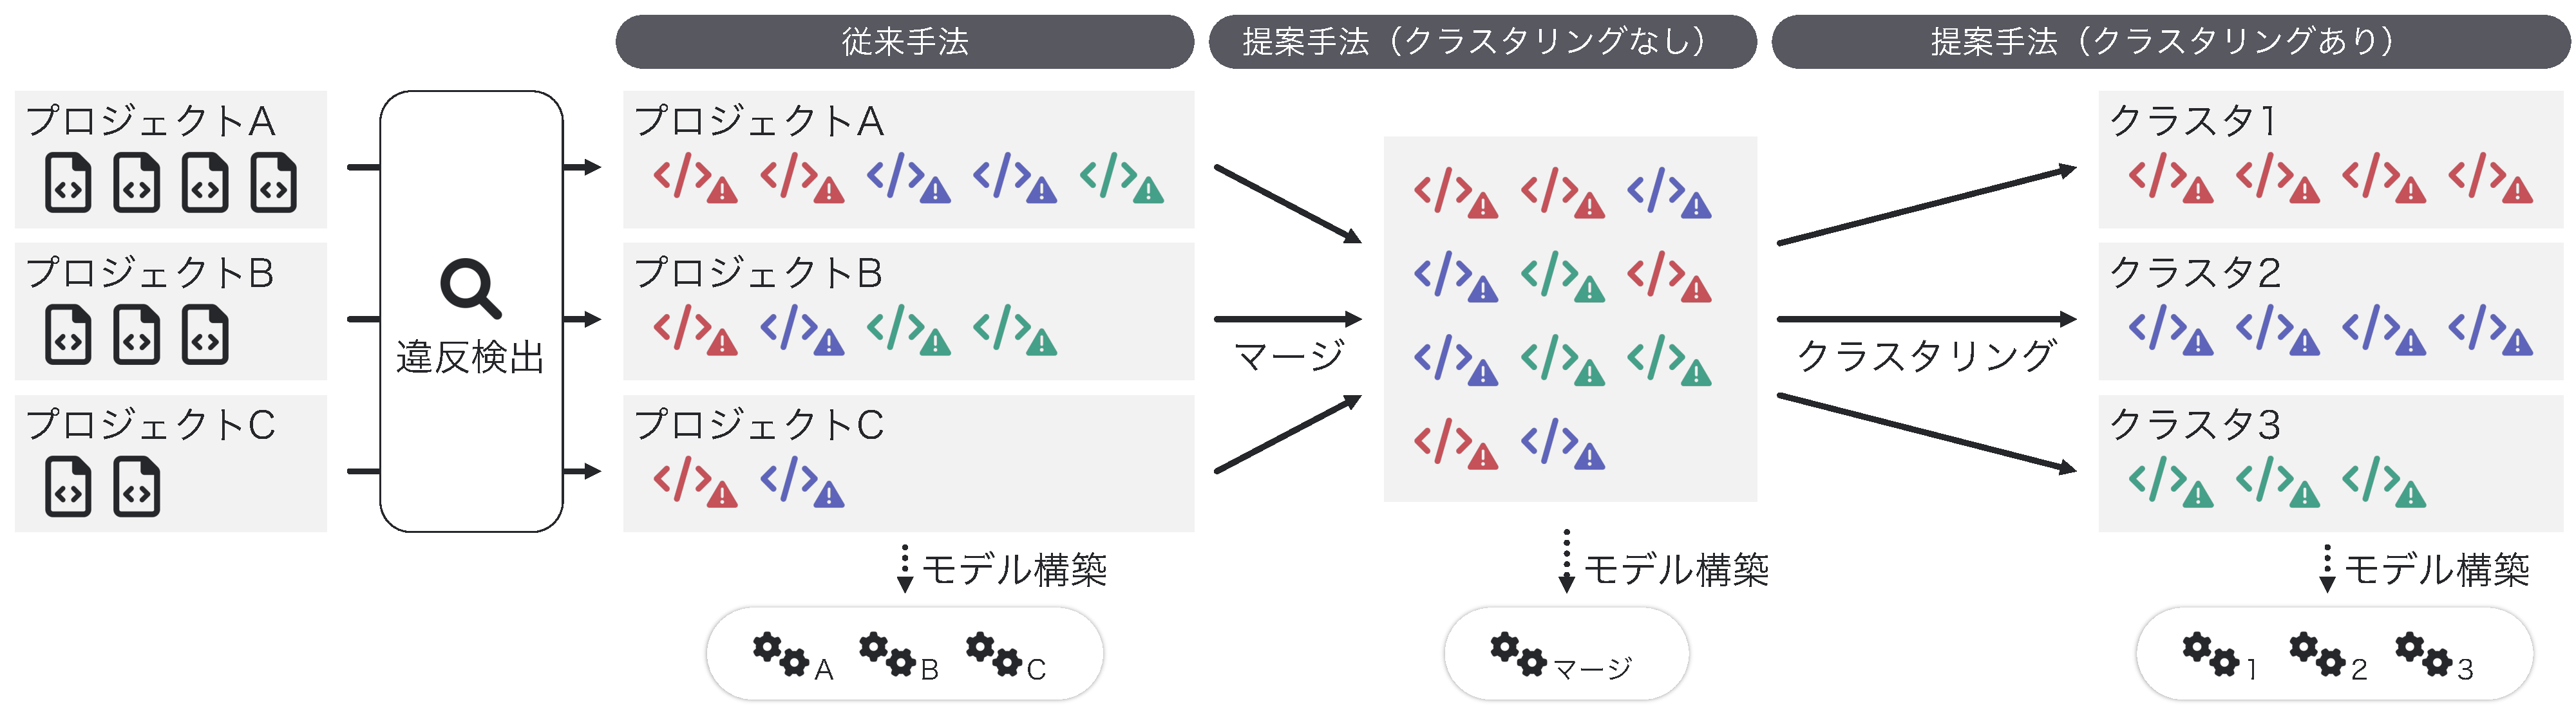
\includegraphics[width=1.0\linewidth]{Kameoka_fig/kameoka_fig1.pdf}
	\caption{本研究の概略図}
	\label{fig:Teiannsyuhou}
\end{figure*}
%------------

図\ref{fig:Teiannsyuhou}は,本研究の提案手法の概略図を示す.本研究では,規約に違反している箇所を修正するか否かを予測する3つの機械学習モデルを構築する.まず,図の左から,各プロジェクトのソースコードを対象に静的解析を行い,規約違反を含むソースコードの特徴量の計測,および,規約違反の修正有無を計測する.次に,学習データとして各プロジェクトの開発履歴のみを用いて機械学習モデル(従来手法)を構築する.続いて,各プロジェクトの開発履歴をすべて統合した学習データを用いた機械学習モデル(提案手法(クラスタリングなし))を構築する.最後に統合した学習データを階層的クラスタリングによって10クラスタに分割し,それぞれのクラスタの開発履歴を用いて機械学習モデル(提案手法(クラスタリングあり))を構築する.本研究では,評価に用いるオープンソースソフトウェアの対象プロジェクト数に合わせてクラスタ数を10としている.また,提案手法のクラスタリングは,全てのプロジェクトの学習データと評価用データを合わせてクラスタリングを行い,評価用データは,分類されたクラスタの学習データで構築したモデルを用いて予測する.


% 本研究では,違反回数の少ない規約であったとしても特定するために,評価対象プロジェクトに加えた複数のプロジェクトの開発履歴を使用することで学習データを拡大する.さらに,規約違反に対する修正の慣習が異なるプロジェクトの開発履歴を用いることによる予測精度の低下を防ぐために,コード断片の特徴量が類似する規約違反しているコード断片をクラスタリングする.各クラスタでそれぞれ予測モデルを構築する.クラスタリングでは,学習データと検証データを統合し,両データのの説明変数に基づき分類することで,検証データが類似する規約違反するコード断片によって生成された機械学習モデルで予測を行えるようにする.予測モデルの構築には各クラスタの学習データのみ使用する.


% 学習データに評価対象とは異なるプロジェクトの開発履歴も使用することにより,違反回数の少ない規約であったとしても特定することができると考える.著者らの知る限り,異なるプロジェクトの開発履歴を用いて修正を要する規約違反ソースコードを特定する手法は確認していない.学習データを増やすことで修正する規約違反のコード断片の特定精度の向上が期待できる.その一方で,組織に応じて実装や違反に対する修正の慣習が異なるため,異なる組織の開発履歴が予測精度の低下を招くことも考えられる.この問題を解決するために,本研究では検証対象とするソースコードと類似する特徴量を有する異なる組織の規約違反を学習する方法を提案する.

% 提案するモデル構築の流れとして,図\ref{fig:Teiannsyuhou}のように,複数プロジェクトの学習データセットを一つに結合し,それぞれのコーディング規約の違反データをクラスタリングを行い,作成されたクラスタごとにそれぞれ機械学習モデルを作成し,修正優先度予測を行う.

\subsection{学習データと評価データの収集}

本研究では,2種類の提案手法において構築する機械学習モデルにおいて複数のプロジェクトの開発履歴を統合するが,モデル構築に使用する学習データにも,検証に使用する評価データにも全てのプロジェクトが含まれるように考慮する.具体的には,各プロジェクトの分析対象期間に発生するコミットのうち,前半8割を学習データ,後半2割を評価データとし,各プロジェクトにおいて未来のデータを含まないようにするため交差検証を行わない.


%ここで,学習データとテスト用データを交差検証を行わない理由は,データセットには,時系列が存在しており,ランダムに学習データとテストデータを分割した場合,学習データに未来の情報を含んでしまうため,データセットの分割時にシャッフルは行わない.

\subsection{説明変数の計測方法}

%-------------------------
\begin{figure}[t]
	\centering
	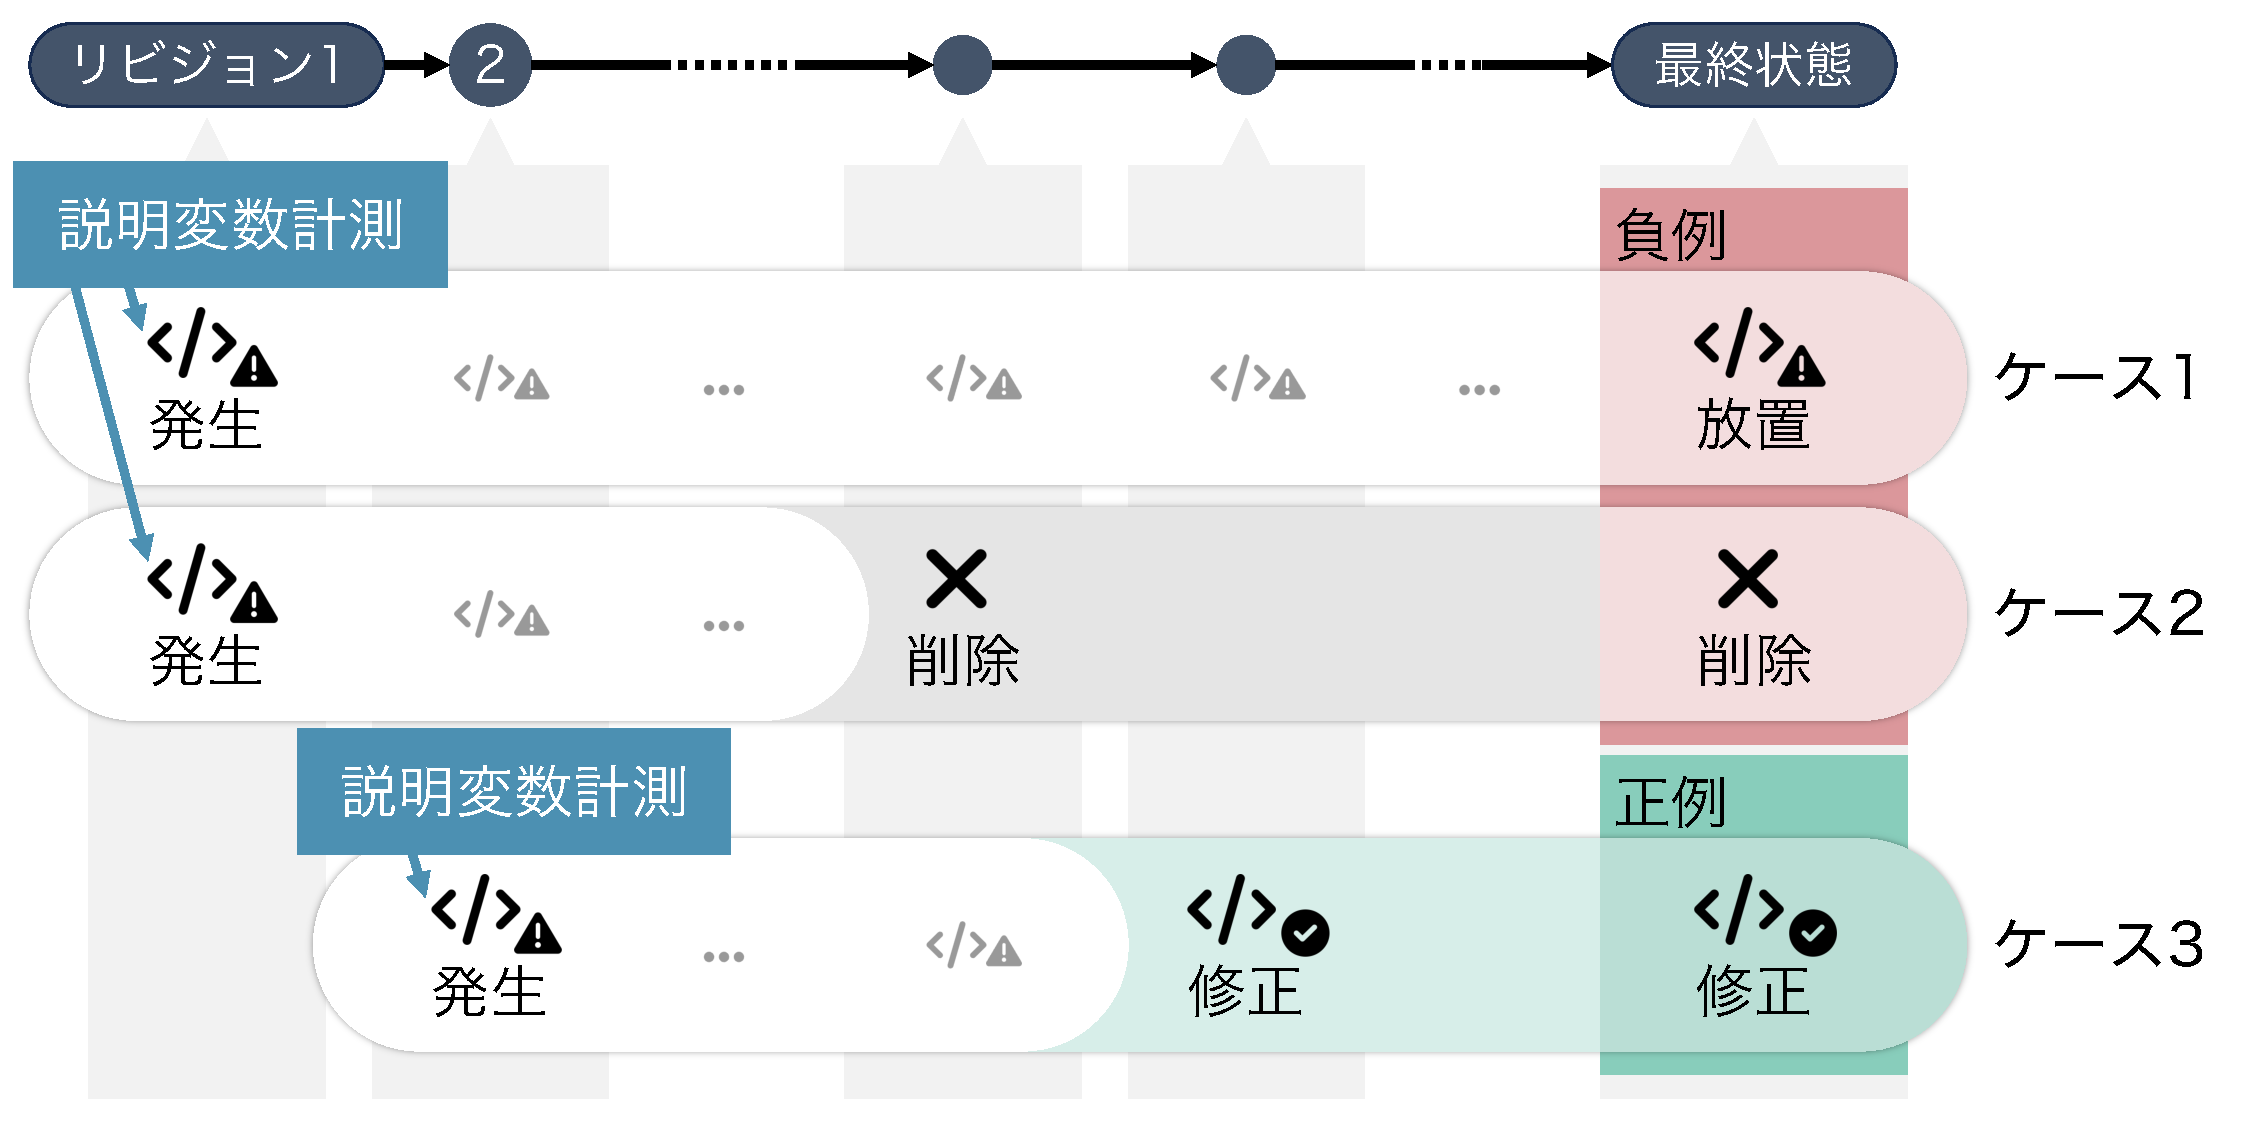
\includegraphics[width=1.0\linewidth]{Kameoka_fig/kameoka_fig2.pdf}
	\caption{説明変数と目的変数の計測方法}
	\label{fig:mokutekihensu}
\end{figure}
%-------------------------

本研究では,分析対象期間中のコミットにおいて変更されたPython言語で記述されたソースコード全てに静的解析ツールを実行する.特定のソースコード断片において初めて規約違反が検出されたコミットを,修正を要するか否かを判定する予測時点とし,説明変数を計測する.

%機械学習モデルの学習,テストに用いる説明変数の計測方法について説明する.まず,説明変数の計測地点について,計測地点はコーディング規約に違反しているコードが生成されたリビジョンである.
図\ref{fig:mokutekihensu}は,説明変数と目的変数の計測事例を示す.この例では,コーディング規約への違反が3箇所で検出され,上2つはリビジョン1で発生し,下の1つはリビジョン2で発生しており,それぞれのリビジョンにおいて説明変数を計測する.説明変数の計測地点において,コーディング規約に違反するコード断片を含むソースコードファイルの関数,クラス,モジュールに対して特徴量をテクマトリックス株式会社が開発する静的解析ツールUnderstand\footnote{Understand: \url{https://www.techmatrix.co.jp/product/understand/}}を用いて計測する.説明変数は,ソースコードの特徴量であるコード行数,コメント行数,循環的複雑度,ネストの深さの最大値など含むソースコードに関する特徴量43種類に,コーディング規約の違反検出時に得られる違反箇所のコード行数1種類,規約違反IDをOne-hotベクトル化した1種類の,合計45種類の特徴量を使用する.

\subsection{目的変数の計測方法}

本研究では,分析対象期間中に修正されるか否かを目的変数とする.分析対象期間中に修正された規約違反のコード断片と修正されないままの規約違反含むコード断片は表\ref{tab:pos_neg}に示すように正例と負例の2クラスに分類する.
%図\ref{fig:mokutekihensu}の例を,本分類に従うと上2つは負例,下1つは正例となる.

%----------------------
\begin{table}[t]
    \centering
    \caption{正例と負例の分類}
    \label{tab:pos_neg}
    \scalebox{0.75}{
    \begin{tabular}{l|l}
         \hline
            分類 & 説明\\ \hline
            負例 & コーディング規約の違反が放置されているコード断片\\
            負例 & コーディング規約に違反していたコード断片が削除された\\
            正例 & コーディング規約に違反していたコード断片が修正された\\
         \hline
    \end{tabular}
    }
\end{table}

% \begin{table*}[t]
%     \centering
%     \caption{使用した説明変数抜粋\todo{いらないかも}}
%     \label{explaneTable}
%     \scalebox{0.7}{
%     \begin{tabular}{c|c|c|c}
%     カテゴリ & 説明変数名称 & 説明 & 数 \\ \hline
%     \hline
%     \multirow{2}{*}{規約違反の情報} & 各規約違反ID & プロジェクトごとに発生している規約違反のIDをOne-hotベクトル化したもの. & プロジェクトによって異なる \\
%      & Line\_Number & 規約違反が発生しているコード行数 & 1個 \\ \hline
%      \hline
%     \multirow{4}{*}{プログラムファイル特徴量}  & MaxNesting & ネストの深さの最大値 & \multirow{4}{*}{計43個}\\ 
%     & CountLine & コード行数 &   \\ 
%     & Cyclomatic & 循環的複雑度 &  \\ 
%     & & など & \\
%     \hline
%     \end{tabular}
%     }
% \end{table*}

%----------------------

% %-------------------------
% \begin{itemize}
%     \item コーディング規約の違反が放置されている:負例
%     \item コーディング規約がなくなっている
%     \begin{itemize}
%         \item コーディング規約に違反していたコードが削除された:負例
%         \item コーディング規約に違反していたコードが修正された:正例
%     \end{itemize}
% \end{itemize}
% %-------------------------


\newpage
\subsection{規約違反しているコード断片のクラスタリング}

本研究では,説明変数の特徴量が類似する規約違反しているコード断片をクラスタリングした後に,各クラスタに分類されたコード断片の学習データを用いてモデルを構築する.クラスタリングには,クラスタ間の類似度を確認するため階層的クラスタリングを用いる.階層的クラスタリングにおける,クラスタ間の距離はユークリッド距離を用い,クラスタの連結法にはWard法を用いる.本研究では検証に10プロジェクトの開発履歴を使用するため,クラスタ数を10とする.階層クラスタリングによって,従来手法で予測できなかったコード断片を分析する.

\subsection{機械学習モデルの構築と評価}

予測モデルの構築には,
Ruthruffらの従来研究と同様にロジスティック回帰モデルを用いる\cite{JyuraiPre}.本研究で取り扱うコーディング規約に違反しているコード断片は,修正されないままのコード断片が多数含まれる不均衡なデータとなっている.したがって,本研究ではロジスティック回帰分析にはPythonパッケージであるsklearnのlinear\_model.LogisticRegression\footnote{https://scikit-learn.org/stable/modules/generated/\\sklearn.linear\_model.LogisticRegression.html}を使用し,パッケージのオプションclass\_weightsを使用することで2クラスデータの分類に重み付けし,不均衡による問題を解決する.また,ロジスティック回帰モデルの学習を行う際にイテレーションの最大値を10,000回に設定する.
%しているが,クラスタ数が少ない場合に,モデルが最後まで収束しないことが起きたため,最後まで収束させた場合の結果とが生じる可能性がある.

予測モデルの予測性能を評価する指標として,従来研究で用いられている適合率,再現率,F1値を使用する.機械学習モデルの予測結果は次の4つに分類することができ,分類結果に基づき各評価指標を算出する.
\begin{itemize}
\item True Positive(TP): 修正された規約違反に対して,修正されると正しく予測するケース
\item False Positive(FP): 放置された規約違反に対して,修正されると誤って予測するケース
\item True Negative(TN):放置された規約違反に対して,放置されると正しく予測するケース
\item False Negative(FN):修正された規約違反に対して,放置されると誤って予測するケース
\end{itemize}
%また,データセットの学習データとテストデータの分割の割合は,リビジョンごとのデータの前8割を学習用データとし,後2割をテスト用データとして用いる.ここで,学習データとテスト用データを交差検証を行わない理由は,データセットには,時系列が存在しており,ランダムに学習データとテストデータを分割した場合,学習データに未来の情報を含んでしまうため,データセットの分割時にシャッフルは行わない.

%クロスプレディクションを行う際に用いる学習データは,従来手法でも用いたデータセットの前8割をクラスタリングし,それぞれのクラスタに属しているものをそのクラスタの機会学習モデルの学習データとすることによって,クラスタごとのモデル構築を行う.


%%%%%%%%%%%%%%%%%%%%%%%%%%%%%%%%%%%%%%
\section{評価実験}\label{sec:result}
%%%%%%%%%%%%%%%%%%%%%%%%%%%%%%%%%%%%%%

\subsection{データセット}
%------------
\begin{table*}[t]
    \centering
    \caption{分析対象プロジェクトの統計量(総違反数で昇順に記載)}
    \label{datasetTB}
    \scalebox{1.0}{
    \begin{tabular}{l|r|r|r|r|r}
         \hline
         \multirow{2}{*}{プロジェクト名} & \multirow{2}{*}{対象リビジョン数} & \multicolumn{1}{c|}{違反修正数} & \multicolumn{1}{c|}{違反放置数}& \multicolumn{1}{c|}{\multirow{2}{*}{総違反数}} & \multicolumn{1}{c}{\multirow{2}{*}{違反修正率}} \\ 
                      &               &\multicolumn{1}{c|}{(正例)} & \multicolumn{1}{c|}{(負例)} &&\\ \hline
         \hline %
python-bugzilla & 243 & 189 & 183 & 372 & 51\%\\
python-cloudant & 657 & 269 & 1,299 & 1,568 & 17\%\\
pynput & 507 & 431 & 3,595 & 4,026 & 11\%\\
pyscard & 380 & 681 & 2,705 & 3,386 & 20\%\\
howdoi & 593 & 721 & 434 & 1,155 & 62\%\\
hickle & 245 & 920 & 1,293 & 2,213 & 42\%\\
transitions & 496 & 1,182 & 2,620 & 3,802 & 31\%\\
OWSLib & 422 & 1,547 & 3,080 & 4,627 & 33\%\\
schema\_salad & 564 & 1,990 & 3,009 & 4,999 & 40\%\\
schematics & 524 & 6,950 & 4,829 & 11,779 & 59\%\\
         \hline
    \end{tabular}
    }
\end{table*}
%------------

%--------------------
\begin{table*}[t]
    \centering
    \caption{予測結果}
    \label{PrevPrediction}
    \begin{tabular}{l|ccc|ccc|ccc}
         \hline
         \multirow{3}{*}{プロジェクト名}&\multicolumn{3}{c|}{\multirow{2}{*}{従来手法}} & \multicolumn{3}{c|}{提案手法} & \multicolumn{3}{c}{提案手法}\\
         &\multicolumn{3}{c|}{} & \multicolumn{3}{c|}{(クラスタリングなし)} & \multicolumn{3}{c}{(クラスタリングあり)}\\ \cline{2-10}
          & 適合率 & 再現率 & F1値 & 適合率 & 再現率 & F1値 & 適合率 & 再現率 & F1値\\ \hline
         \hline %
            python-bugzilla & 0.54 & 0.13 & 0.21 & \textbf{\underline{0.69}} & \textbf{\underline{0.64}} & \textbf{\underline{0.67}} & 0.63 & 0.23 & 0.33\\
            python-cloudant & \textbf{\underline{0.77}} & \textbf{\underline{0.81}} & \textbf{\underline{0.79}} & 0.17 & 0.17 & 0.17 & 0.65 & 0.32 & 0.43\\
            pynput & 0.41 & \textbf{\underline{0.94}} & 0.58 & 0.42 & 0.71 & 0.53 & \textbf{\underline{0.57}} & 0.65 & \textbf{\underline{0.61}}\\
            pyscard & \textbf{\underline{0.29}} & \textbf{\underline{0.91}} & \textbf{\underline{0.44}} & 0.18 & 0.89 & 0.30 & 0.12 & 0.41 & 0.18\\
            howdoi & 0.92 & \textbf{\underline{0.96}} & \textbf{\underline{0.94}} & \textbf{\underline{0.93}} & 0.59 & 0.72 & \textbf{\underline{0.93}} & 0.51 & 0.66\\
            hickle & 0.33 & \textbf{\underline{0.73}} & 0.45 & 0.36 & 0.66 & \textbf{\underline{0.47}} & \textbf{\underline{0.41}} & 0.47 & 0.44\\
            transitions & \textbf{\underline{0.80}} & \textbf{\underline{0.87}} & \textbf{\underline{0.83}} & 0.68 & 0.50 & 0.57 & 0.68 & 0.21 & 0.32\\
            OWSLib & \textbf{\underline{0.84}} & 0.86 & \textbf{\underline{0.85}} & 0.76 & \textbf{\underline{0.92}} & 0.83 & 0.83 & 0.88 & \textbf{\underline{0.85}}\\
            schema\_salad & \textbf{\underline{0.52}} & \textbf{\underline{0.66}} & \textbf{\underline{0.58}} & 0.21 & 0.52 & 0.30 & 0.15 & 0.21 & 0.17\\
            schematics & \textbf{\underline{0.30}} & 0.79 & \textbf{\underline{0.44}} & 0.26 & \textbf{\underline{0.94}} & 0.41 & 0.27 & 0.84 & 0.40\\
    \hline
    \end{tabular}
\end{table*}
%--------------------


%--------------------------
\begin{table*}[t]
    \centering
    \caption{従来手法の予測結果分析}
    \label{PrevPredictionCrustering}
    \scalebox{0.67}{
    \begin{tabular}{l|c|c|c|c|c|c|c|c|c|c}
         \hline
         プロジェクト名 & cluster 1 & cluster 2 & cluster 3 & cluster 4 & cluster 5 & cluster 6 & cluster 7 & cluster 8 & cluster 9 & cluster 10\\ \hline
         \hline %
         python-bugzilla & \textbf{\underline{0.67}}* & -- & 0.33* & -- & 0.13* & -- & --* & -- & -- & -- \\ \hline
         python-cloudant & \textbf{\underline{0.95}}* & -- & \textbf{\underline{0.89}}* & -- & 0.89* & -- & \textbf{\underline{0.97}}* & -- & -- & -- \\ \hline
         pynput & 0.70* & -- & 0.35* & -- & -- & -- & -- & -- & -- & \textbf{\underline{1.00}}* \\ \hline
         pyscard & \textbf{\underline{0.76}}* & \textbf{\underline{1.00}}* & \textbf{\underline{0.78}}* & -- & -- & --* & -- & -- & \textbf{\underline{1.00}}* & -- \\ \hline
         howdoi & 0.57* & -- & \textbf{\underline{0.91}}* & -- & -- & -- & -- & -- & -- & -- \\ \hline
         hickle & -- & -- & 0.51* & -- & -- & -- & -- & -- & -- & -- \\ \hline
         transitions & \textbf{\underline{0.82}}* & -- & \textbf{\underline{0.86}}* & -- & --* & -- & \textbf{\underline{0.80}}* & -- & -- & -- \\ \hline
         OWSLib & 0.94* & \textbf{\underline{1.00}}* & \textbf{\underline{0.80}}* & -- & \textbf{\underline{1.00}}* & -- & \textbf{\underline{0.87}}* & \textbf{\underline{1.00}}* & -- & -- \\ \hline
         schema\_salad & \textbf{\underline{0.72}}* & -- & \textbf{\underline{0.86}}* & 0.62* & \textbf{\underline{0.92}}* & -- & 0.26* & -- & -- & -- \\ \hline
         schematics & \textbf{\underline{0.47}}* & -- & \textbf{\underline{0.47}}* & -- & -- & -- & \textbf{\underline{0.56}}* & -- & -- & -- \\
         \hline
    \end{tabular}
    }

\vspace{1mm}

    \centering
    \vspace{1mm}
    \caption{提案手法(クラスタリングなし)の予測結果分析}
    \label{MergePredictionCrustering}
    \scalebox{0.67}{
    \begin{tabular}{l|c|c|c|c|c|c|c|c|c|c}
         \hline
         プロジェクト名 & cluster 1 & cluster 2 & cluster 3 & cluster 4 & cluster 5 & cluster 6 & cluster 7 & cluster 8 & cluster 9 & cluster 10\\ \hline
         \hline %
         python-bugzilla & \textbf{\underline{0.67}}* & -- & \textbf{\underline{0.42}}* & -- & \textbf{\underline{1.00}}* & -- & --* & -- & -- & -- \\ \hline
         python-cloudant & 0.71* & -- & 0.72* & -- & 0.73* & -- & 0.73* & -- & -- & -- \\ \hline
         pynput & 0.57* & -- & 0.56* & -- & -- & -- & -- & -- & -- & \textbf{\underline{1.00}}* \\ \hline
         pyscard & 0.58* & \textbf{\underline{1.00}}* & 0.60* & -- & -- & --* & -- & -- & \textbf{\underline{1.00}}* & -- \\ \hline
         howdoi & 0.57* & -- & 0.62* & -- & -- & -- & -- & -- & -- & -- \\ \hline
         hickle & -- & -- & 0.59* & -- & -- & -- & -- & -- & -- & -- \\ \hline
         transitions & 0.69* & -- & 0.60* & -- & --* & -- & 0.52* & -- & -- & -- \\ \hline
         OWSLib & 0.91* & \textbf{\underline{1.00}}* & 0.75* & -- & \textbf{\underline{1.00}}* & -- & 0.85* & \textbf{\underline{1.00}}* & -- & -- \\ \hline
         schema\_salad & 0.54* & -- & 0.09* & \textbf{\underline{0.78}}* & 0.03* & -- & \textbf{\underline{0.78}}* & -- & -- & -- \\ \hline
         schematics & 0.20* & -- & 0.34* & -- & -- & -- & 0.45* & -- & -- & -- \\
         \hline
    \end{tabular}
    }

    
\vspace{1mm}
    \centering
    \vspace{1mm}
    \caption{提案手法(クラスタリングあり)の予測結果分析}
    \label{AproPredictionCrustering}
    \scalebox{0.67}{
    \begin{tabular}{l|c|c|c|c|c|c|c|c|c|c}
         \hline
         プロジェクト名 & cluster 1 & cluster 2 & cluster 3 & cluster 4 & cluster 5 & cluster 6 & cluster 7 & cluster 8 & cluster 9 & cluster 10\\ \hline
         \hline %
         python-bugzilla & \textbf{\underline{0.67}}* & -- & 0.37* & -- & 0.27* & -- & --* & -- & -- & -- \\ \hline
         python-cloudant & 0.90* & -- & 0.77* & -- & \textbf{\underline{0.91}}* & -- & 0.73* & -- & -- & -- \\ \hline
         pynput & \textbf{\underline{0.80}}* & -- & \textbf{\underline{0.64}}* & -- & -- & -- & -- & -- & -- & \textbf{\underline{1.00}}* \\ \hline
         pyscard & 0.63* & \textbf{\underline{1.00}}* & 0.64* & -- & -- & --* & -- & -- & \textbf{\underline{1.00}}* & -- \\ \hline
         howdoi & 0.57* & -- & 0.55* & -- & -- & -- & -- & -- & -- & -- \\ \hline
         hickle & -- & -- & \textbf{\underline{0.67}}* & -- & -- & -- & -- & -- & -- & -- \\ \hline
         transitions & 0.61* & -- & 0.21* & -- & --* & -- & 0.53* & -- & -- & -- \\ \hline
         OWSLib & \textbf{\underline{0.95}}* & \textbf{\underline{1.00}}* & \textbf{\underline{0.80}}* & -- & \textbf{\underline{1.00}}* & -- & 0.86* & \textbf{\underline{1.00}}* & -- & -- \\ \hline
         schema\_salad & 0.44* & -- & 0.51* & 0.62* & 0.03* & -- & 0.22* & -- & -- & -- \\ \hline
         schematics & 0.23* & -- & 0.42* & -- & -- & -- & 0.55* & -- & -- & -- \\
         \hline
    \end{tabular}
    }

\vspace{1mm}
    \centering
    \vspace{1mm}
    \caption{各クラスタが保有するデータ数(k=10)}
    \label{CrusteringDataNum}
    \scalebox{0.67}{
    \begin{tabular}{l|c|c|c|c|c|c|c|c|c|c}
         \hline
         プロジェクト名 & cluster 1 & cluster 2 & cluster 3 & cluster 4 & cluster 5 & cluster 6 & cluster 7 & cluster 8 & cluster 9 & cluster 10\\ \hline
         \hline %
         python-bugzilla & 65* & -- & 80* & -- & 65* & -- & 97* & -- & -- & -- \\ \hline
         python-cloudant & 473* & -- & 455* & -- & 181* & -- & 145* & -- & -- & -- \\ \hline
         pynput & 489* & -- & 299* & -- & -- & -- & -- & -- & -- & 2,432* \\ \hline
         pyscard & 334* & 204* & 2,053* & -- & -- & 71* & -- & -- & 46* & -- \\ \hline
         howdoi & 223* & -- & 701* & -- & -- & -- & -- & -- & -- & -- \\ \hline
         hickle & -- & -- & 1,770* & -- & -- & -- & -- & -- & -- & -- \\ \hline
         transitions & 1,261* & -- & 655 & -- & 417* & -- & 708* & -- & -- & -- \\ \hline
         OWSLib & 574* & 37* & 2,443* & -- & 83 & -- & 555* & 9* & -- & -- \\ \hline
         schema\_salad & 1,019* & -- & 1,139* & 871* & 385* & -- & 585* & -- & -- & -- \\ \hline
         schematics & 2,959* & -- & 4,860* & -- & -- & -- & 1,604* & -- & -- & -- \\
         \hline
    \end{tabular}
    }
\end{table*}
%---------------------

本研究ではケーススタディとして,Libraries.io\footnote{Libraries.io: \url{https://libraries.io/}}からPython言語で実装され,静的解析ツールPylintを開発に使用しているプロジェクトを対象とする.当該プロジェクトの中でstar数が上位の100プロジェクトから,コーディング規約違反の修正割合が高い10プロジェクト(transitions, schematics, schema\_salad, python-bugzilla, python-cloudant, pyscard, pynput, OWSLib, howdoi, hickle)を対象とする.すべてのプロジェクトがGitHubによってソフトウェア,および開発履歴を公開している.本研究では,各分析対象プロジェクトにおいて,2018年12月から1,000日間のコミット履歴を分析対象とする.表\ref{datasetTB}は,各プロジェクトに関する開発履歴の統計量を(総違反数で照準に記載)示す.本研究では,コーディング規約違反の修正割合が高いプロジェクトを選定しているが,修正割合はプロジェクトによって大きく異なる.

\subsection{結果}

本研究では,学習データに評価対象とは異なるプロジェクトの開発履歴も使用することにより,違反回数の少ない規約であったとしても特定するモデルを構築する.本手法の有効性を評価するために3種類のモデルを構築し,比較する.
\begin{itemize}
\item \textbf{従来手法}:評価対象プロジェクトと同じプロジェクトの開発履歴を学習するモデル
\item \textbf{本手法(クラスタリングなし)}:評価対象プロジェクトを含めた10プロジェクトの開発履歴を学習するモデル
\item \textbf{本手法(クラスタリングあり)}:評価対象プロジェクトを含めた10プロジェクトの開発履歴を,説明変数が類似するクラスタに分割し,それぞれのクラスタで学習するモデル
\end{itemize}

表\ref{PrevPrediction}は,従来手法,提案手法(クラスタリングなし),提案手法(クラスタリングあり)により構築した予測モデルの結果を示す.各プロジェクトにおいて3つの手法の中で最も予測性能の高い手法は太字と下線で示す.

\noindent\textbf{知見1: 複数プロジェクトの開発履歴を用いて構築した予測モデルの性能が,評価対象とするプロジェクトの過去の開発履歴のみを用いて構築した予測モデルよりも高い性能になるプロジェクトがある.}

各プロジェクトのF1値に着目すると,2プロジェクト(python-bugzilla,hickle)は従来手法よりも提案手法(クラスタリングなし)のほうが予測性能が高く,2プロジェクト(pynput,OWSLib)は従来手法と比べて,提案手法(クラスタリングあり)と同等,またはそれよりも予測性能が高く.複数のプロジェクトを使用したとしても精度が下がらないケースもあることを確認した.その他の6プロジェクトは従来手法のほうが予測性能が高かった.

\noindent\textbf{知見2: 学習データの少ないプロジェクト(python-bugzilla)は複数プロジェクトの開発履歴を用いることで,従来手法より高い精度で予測できる.}

python-bugzillaは,従来手法のF1値が0.21であるが,提案手法(クラスタリングなし)と提案手法(クラスタリングあり)のF1値がそれぞれ0.67と0.33となり,複数プロジェクトの開発履歴を用いることにより精度が向上することが明らかとなった.提案手法(クラスタリングあり)は,クラスタリングすることによって学習データの不足を緩和するものと示唆される.pynputは正例が極端に少ないため,提案手法(クラスタリングなし)により十分な学習データを使用でき,予測性能が向上したと示唆される.

一方,python-bugzillaほどではないがデータサイズの小さいhowdoiや,正例の少ないpython-cloudantは提案手法で他のプロジェクトを学習することにより予測性能が低下した.
また,hincleとOWSLibは従来手法と同じ精度,または提案手法の方が予測性能の向上はわずかであるため,効果があるとは言えない.\\




% 本手法の有効性を評価するために,2つのリサーチクエスチョン (RQ) に回答する.
% \begin{itemize}
%     \item RQ1 従来研究で修正予測できなかったデータの特徴とは
%     \item RQ2 クロスプレディクションを行った場合,従来研究で予測できなかった修正予測ができるのか
% \end{itemize}
% \vspace{0.2\baselineskip}  % 余白の調整
%
%RQ1では,従来手法で予測できていないデータの分析を行う.分析内容は,提案アプローチであるクラスタリングを行った結果を用いて,予測できなかったデータがどのクラスタに含まれるのかを確認する.予測できていないデータがそのプロジェクトが保持するデータの中で少数クラスタに存在すれば,提案アプローチが有効である可能性が考えられる.
%
%RQ2では実際に提案アプローチで構築した機械学習モデルの有効性を評価する.評価方法として修正優先度予測を行い,その適合率,再現率,F1値,正解率を比較することによって評価する.

続いて,表\ref{AproPredictionCrustering}は,本研究の提案手法において10のクラスタに分類したときの,クラスタ別の性能(正解率)を示す.また,表\ref{PrevPredictionCrustering},表\ref{MergePredictionCrustering}はそれぞれ提案手法(クラスタリングあり)と同じ評価データが,従来手法のモデルと提案手法(クラスタリングなし)のモデルを用いた場合の予測性能の結果を示す.セル中の``--''は,評価用データが当該クラスタに存在しなかったことを示す.表\ref{PrevPredictionCrustering},\ref{MergePredictionCrustering},\ref{AproPredictionCrustering}の`` * ''は,学習時にデータが存在していたことを示し,表\ref{CrusteringDataNum}と合わせて見ると,python-bugzillaのcluster 7は97個の学習データが存在するが,評価用データにはデータがないため,予測結果の分析を行った表には`` --* ''で表示されている.
% \todo{理解できない}
cluster 1とcluster 2は精度が他に比べて高く,"--"が多いことがわかる.これは,どのプロジェクトでも類似度が高いファイルがクラスタ0, 2に集約され,プロジェクトの差が出る他クラスタは,単一プロジェクト内でしか類似性が無いことを示している.

% \todo{知見3と4は後ほど修正}


\noindent\textbf{知見3: 特定のクラスタのみで性能が向上するプロジェクトがある.}

python-bugzillaにおいてcluster 1では,他のプロジェクトの開発履歴を用いた場合と同程度の予測性能を確認できる.また,cluster 3とcluster 5は,従来手法に比べて提案手法の予測性能が向上した.sceme\_saladでは,表\ref{PrevPrediction}において従来手法の方が提案手法よりも精度が高いが,cluster 4では従来手法よりも提案手法(クラスタリングなし)の方が予測性能が高い.cluster 4は,コード行数や循環的複雑度などの中央値が他のクラスタの中央値と比較して5倍程度大きく,大規模なファイルが多く集まっているクラスタである.従来手法では,過去の開発履歴において全てのデータを用いて学習しており,特定のクラスタに属する規約違反の予測に寄与しないデータも含まれていたため予測性能が低下していることが示唆される.
% \todo{cluster4が何か書きたい.}
hickleでは,表\ref{PrevPrediction}において従来手法の方が提案手法よりも高い予測性能であるが,cluster 3においてのみ提案手法(クラスタリングあり)が従来手法よりも高い予測性能となっている.

\noindent\textbf{知見4: 従来手法(評価対象プロジェクトの過去の開発データのみ用いたモデル)が提案手法に比べて高い性能となることもある.}

cluster 1やcluster 2は,分析対象とする全てのプロジェクトの規約違反を含んでおり,hickleのように高い精度となる場合もあるが,一方で,異なるプロジェクトを学習することで性能が低下するプロジェクトが多い.




%表\ref{PrevPredictionCrustering}について詳細に言及すると,cluster\_4のpython-bugzillaは,他プロジェクトのcluster\_4の結果と比較して精度が低いことがわかる.cluster\_4のpython-bugzillaのテストデータは15件存在しており,そのうち2件しか正解していない.また,python-bugzillaは全体的な精度も低い.原因として,ほかのデータセットと比較して全体のコミット数が少なく,ロジスティック回帰のモデルが十分に学習できなかったが考えられる.このような事象に対して,本研究のアプローチである,クラスタリングの結果に基づいて他プロジェクトのデータも含めて学習を行うことで学習データを保管すれば精度向上を見込むことができる.

%多くのデータが含まれるcluster\_0とcluster\_2は,自プロジェクトの他のクラスタに属する予測結果と比較して予測精度が低下していることがわかる.これは,互いに修正優先度の予測に有効なパラメータを相殺してしまっていると考えられる.




%\subsection{RQ1 従来研究で修正予測できなかったデータの特徴とは}
% \begin{table}[tb]
%     \centering
%     \caption{従来手法による修正優先度予測結果}
%     \label{PrevPrediction}
%     \begin{tabular}{|l|c|c|c|c|}
%          \hline
%          プロジェクト名 & 適合率 & 再現率 & F1値 & 正解率 \\ \hline
%          \hline %
%          pynput & 0.41 & 0.94 & 0.58 & 0.86 \\ \hline
%          pyscard & 0.29 & 0.91 & 0.44 & 0.78 \\ \hline
%          howdoi & 0.92 & 0.96 & 0.94 & 0.90 \\ \hline
%          schema\_salad & 0.52 & 0.66 & 0.58 & 0.74 \\ \hline
%          python-bugzilla & 0.54 & 0.13 & 0.21 & 0.31 \\ \hline
%          OWSLib & 0.84 & 0.86 & 0.85 & 0.82 \\ \hline
%          python-cloudant & 0.77 & 0.81 & 0.79 & 0.93 \\ \hline
%          hickle & 0.33 & 0.73 & 0.45 & 0.50 \\ \hline
%          transitions & 0.80 & 0.87 & 0.83 & 0.82 \\ \hline
%          schematics & 0.30 & 0.79 & 0.44 & 0.50 \\
%          \hline
%     \end{tabular}
% \end{table}

% 表\ref{PrevPrediction}は,従来手法による修正優先度予測の結果である.F1値が0.21から0.94まで幅広く存在しており,修正優先度予測の結果が安定していないことがわかる.この結果の原因を追求するために,それぞれの保有しているデータが,すべてのプロジェクト全体でどのような類似性があるファイルを使っているかを追求した.






% \subsection{RQ2 クロスプレディクションを行った場合,従来研究で予測できなかった修正予測ができるのか}
% \subsubsection{従来手法の結果との比較}
% \begin{table}[tb]
%     \centering
%     \caption{提案手法による修正優先度予測結果(k=10)}
%     \label{AproachPrediction}
%     \begin{tabular}{|l|c|c|c|c|}
%          \hline
%          プロジェクト名 & 適合率 & 再現率 & F1値 & 正解率 \\ \hline
%          \hline %
%             pynput & 0.57 & 0.65 & 0.61 & 0.71 \\
%             pyscard & 0.12 & 0.41 & 0.18 & 0.64 \\
%             howdoi & 0.93 & 0.51 & 0.66 & 0.55 \\
%             schema\_salad & 0.15 & 0.21 & 0.17 & 0.44 \\
%             python-bugzilla & 0.63 & 0.23 & 0.33 & 0.36 \\
%             OWSLib & 0.83 & 0.88 & 0.85 & 0.82 \\
%             python-cloudant & 0.65 & 0.32 & 0.43 & 0.86 \\
%             hickle & 0.41 & 0.47 & 0.44 & 0.67 \\
%             transitions & 0.68 & 0.21 & 0.32 & 0.54 \\
%             schematics & 0.27 & 0.84 & 0.40 & 0.38 \\
%          \hline
%     \end{tabular}
% \end{table}

% 表\ref{AproachPrediction}は提案手法である,データセットを一度結合し,クラスタリングの結果に基づいて予測を行った結果の表である.従来手法と比較して10プロジェクト中2プロジェクトでF1値の向上が確認できる.向上したプロジェクトはpython-bugzillaとpynputの2プロジェクトである.このうちpython-bugzillaはRQ1で考察したようにデータセットサイズが小さく,負例が大半を占めているため,提案手法によるデータセットの補完によって精度が向上したと考えられる.しかし,pynputプロジェクトのデータ数はほかのプロジェクトと比較して多いが,F1値は向上している.pynputプロジェクトの他のプロジェクトと異なる点は,正例の割合が0.11であることである.本研究で用いているロジスティック回帰モデルの構築方法は,オプションとして正例と負例の予測割合が等しくなるように重みづけを行っているため,従来手法のモデル構築方法では,重みづけが過度に発生するため予測精度が低下してしまい,提案手法によって過度の重みづけが解消され予測精度が向上したと考えられる.

% \subsubsection{クラスタリングせずに全てのデータを学習データとした場合との結果の比較}
% \begin{table}[tb]
%     \centering
%     \caption{全てのデータセットをマージした学習データを利用した予測結果}
%     \label{AllPrediction}
%     \begin{tabular}{|l|c|c|c|c|}
%          \hline
%          プロジェクト名 & 適合率 & 再現率 & F1値 & 正解率 \\ \hline
%          \hline %
%             pynput & 0.42 & 0.71 & 0.53 & 0.87 \\
%             pyscard & 0.18 & 0.89 & 0.30 & 0.60 \\
%             howdoi & 0.93 & 0.59 & 0.72 & 0.61 \\
%             schema\_salad & 0.21 & 0.52 & 0.30 & 0.31 \\
%             python-bugzilla & 0.69 & 0.64 & 0.67 & 0.55 \\
%             OWSLib & 0.76 & 0.92 & 0.83 & 0.78 \\
%             python-cloudant & 0.17 & 0.17 & 0.17 & 0.72 \\
%             hickle & 0.36 & 0.66 & 0.47 & 0.59 \\
%             transitions & 0.68 & 0.50 & 0.57 & 0.62 \\
%             schematics & 0.26 & 0.94 & 0.41 & 0.32 \\
%          \hline
%     \end{tabular}
% \end{table}

% 表\ref{AllPrediction}は,機械学習モデルを構築する際に10プロジェクトの全ての学習データセットを,無秩序にマージしたものを学習データとして,それぞれのプロジェクトのテストデータを予測した結果である.この表と従来手法と提案手法の表である表\ref{PrevPrediction},\ref{AproachPrediction}の結果と比較すると従来手法より2プロジェクト,提案手法より6プロジェクトにおいて結果のF1値が向上していた.この結果は,仮説として立てていた「無秩序なデータセットの結合では,修正の特徴が大多数のデータに相殺され予測精度が低下する.」ことに矛盾する. 




\section{考察}\label{sec:consideration}
提案手法として複数プロジェクトの開発履歴を学習に使用することによって,次の特定の状況下において予測精度が向上することが明らかとなった.
% \todo{この条件下でも精度上がらない,維持しない場合があるかは要確認}

\begin{itemize}
    \item 全体的な学習データ数が少ない場合
    \item 修正される(正例)の割合が非常に低い場合
\end{itemize}

従来手法は,学習データ不足のため予測性能が低いという課題があり,python-bugzillaプロジェクトでは本研究における提案手法(クラスタリングなし)においてデータの類似性を問わず複数のプロジェクトの開発履歴を学習することにより正例の割合が増加したことが予測性能の向上に寄与したと示唆される.ただし,正例の割合が小さいプロジェクトとして,pynput(正例割合11\%)では予測性能が向上しているが,python-cloudant(正例割合17\%)では提案手法の予測精度が低下している.このような結果の理由の一つとして,python-cloudantは,クラスタリング結果がpynputと比較して多くのクラスタに分かれていることが考えられる.多数のクラスタに分かれたことによってプロジェクト特有の修正に関する特徴を学習できず,予測性能の低下につながったと示唆される.
% \todo{正例が増加したか否かって確認できる?}

一方で,一部のプロジェクトではクラスタリングによる学習データの分割がクラスタリングなしよりも予測性能が低くなる結果を確認した.その原因として,本研究では学習データを10のクラスタに分割したことで,cluster 1とcluster 3にはデータが偏ったことで違反修正の特徴が汎化されたモデルを生成し,その他のクラスタには少数のデータのみが分類され学習データが不足したことにより予測性能が低下したことが示唆される.

% % --------------------------------
% \begin{figure}[t]
% 	\centering
% 	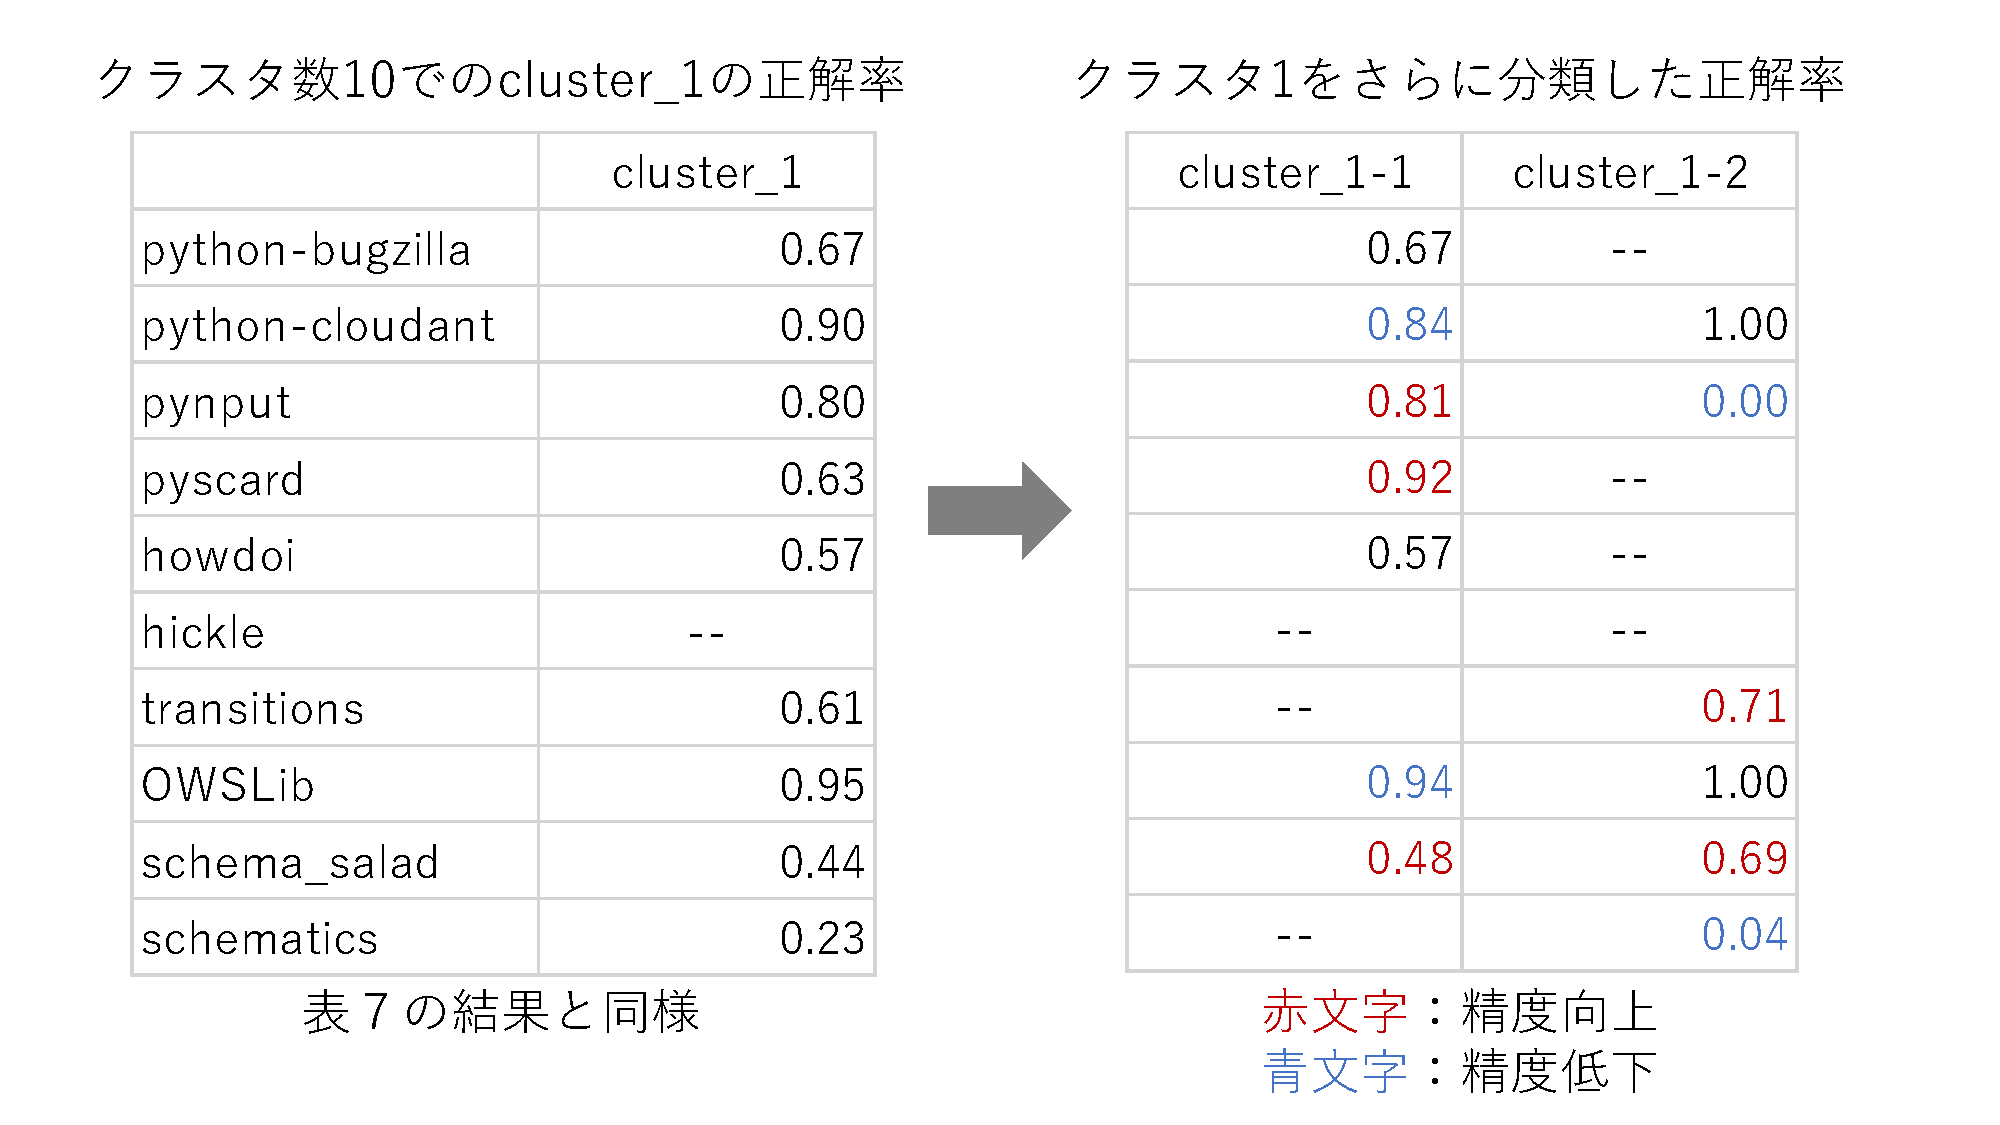
\includegraphics[width=1.0\linewidth]{Kameoka_fig/kosatsu.pdf}
% 	\caption{クラスタ数の変化による予測精度への影響}
% 	\label{fig:kosatsu}
% \end{figure}
% % --------------------------------
%--------------------------
\begin{table}[t]
%    \centering
    \caption{クラスタ数の変化による予測精度への影響}
    \label{MoreCrustering}
    \scalebox{0.8}{
    \begin{tabular}{l|ccc|c}
        \cline{1-2}\cline{4-5}
        & cluster 1 &  & cluster 1-1 & cluster 1-2 \\ \cline{1-2}\cline{4-5}
        python-bugzilla & 0.67 & & 0.67 & -- \\
        python-cloudant & 0.90 & & 0.84 & \textbf{\underline{1.00}} \\
        pynput & 0.80 & & \textbf{\underline{0.81}} & 0.00 \\
        pyscard & 0.63 && \textbf{\underline{0.92}} & -- \\
        howdoi & 0.57 & $\Rightarrow$ & 0.57 & -- \\
        hickle & -- && -- & -- \\
        transitions & 0.61 && -- & \textbf{\underline{0.71}} \\
        OWSLib & 0.95 & & 0.94 & \textbf{\underline{1.00}} \\
        schema\_salad & 0.44 & & \textbf{\underline{0.48}} & \textbf{\underline{0.69}} \\
        schematics & 0.23 & & -- & 0.04\\
        \cline{1-2}\cline{4-5}
    \end{tabular}
    }
\end{table}
%---------------------


この課題解決の方策として,階層的クラスタリングにおいて,特定の深さで枝切りを行うのではなく,クラスタごとに枝切りの深さを変化することで規約違反の特徴を捉えることができると示唆される.具体的には,cluster 1とcluster 3はさらに分割し,その他のclusterは統合することが考えられる.表\ref{MoreCrustering}は,表\ref{AproPredictionCrustering}のcluster 1を2クラスタに分類し,クラスタ数11で予測を行った結果の比較をしている.cluster 1は,コード行数の中央値は他のクラスタの2倍程度であるが,循環的複雑度が8倍になっており,
%循環的複雑度は40を超えるとテスト不可のような指標があるので,
cluster 1には極めて複雑なソースコードも含まれている.従って,cluster 1をcluster 1-1,cluster 1-2に分割することにより多くのプロジェクトで予測性能が向上することを確認した.今後は,データ数が偏っているクラスタの分割や,データ数が極めて少ないクラスタの統合を検討し,予測精度の向上を目指す.





%従来手法は,モデル構築手法は学習データ不足の点から,うまく学習できず,データの類似性を問わず他プロジェクトのデータを結合することによって適度な正例割合を持つ学習データを確保するほうが予測に有効である.クラスタリングによる学習データセットの分割が予測に悪影響を与えた原因として,本研究では,クラスタ数10の場合で検証を行っており,一部のクラスタにデータが集まり,その他クラスタに少数のデータがクラスタリングされた.その結果データ数が多いクラスタは,それぞれのプロジェクトごとに存在する違反修正の特徴が汎化され,データ数が少ないクラスタは学習データが足りずに予測精度が下がってしまったと考えられる.
%この問題を解決するための今後の展望として,階層的クラスタリングを行った際に,ある深さで一直線に枝切りを行うのではなく,クラスタごとに恣意的に枝切りの場所を変化させて予測を行うことによって予測精度を向上させることができると考えられる.



\section{妥当性への脅威}\label{sec:heuristic}
\subsection{内的妥当性}
%表\ref{AproPredictionCrustering}の予測結果は,クラスタ数10にクラスタリングし,それぞれの予測モデルを作成した場合の予測結果であるが,クラスタリングされた学習データセット内に正例あるいは負例のどちらかしか存在しないケースもわずかに存在している.場合,機械学習モデルは構築できず,予測をせずに学習データに含まれているラベルを返すような手法をとっているため,データ数をさらに増やした際に予測精度が変化する可能性がある.

提案手法または,クラスタリングを行わずに複数プロジェクトの開発履歴を統合することによって学習データを拡大した.各プロジェクトにおいてデータセットの分割では時系列を考慮しているが,プロジェクト間では時系列の順序を考慮していない.プロジェクト間においても時系列を考慮した学習データを作成することは今後の課題である.



\subsection{外的妥当性}

本研究ではケーススタディとして10プロジェクト分のデータを学習し予測を行ったが,データセットを拡張することによって正例が増加し予測性能が向上することも示唆されるが,一方で,学習データ増加により各クラスタで作成したモデルが汎化することも考えられる.今後は,プロジェクト数,クラスタ数の適性についても検討する.


\section{おわりに}\label{sec:end}
本研究では,静的解析ツールによって大量に検出されるコーディング規約に違反しているコード断片の中から,優先して修正すべき違反の予測を,複数プロジェクトのデータを結合し,類似性に基づいてクラスタリングしたデータセットを用いることによる予測精度への影響を明らかにした.検証の結果,予測精度だけを見れば,単一プロジェクトのデータだけを用いて学習するほうが予測に効果的であった.今後は考察でも述べたように,多くのデータを保有するクラスタをさらに分割することや,データ数の少ないクラスタ同士の結合によって修正予測精度の向上を目指し,複数プロジェクトのデータを機械学習モデルに学習させる手法の有効性を明らかにする.

%\textbf{謝辞}\

%\textbf{ありがとうございます.}

% 本フォーマットの基になったスタイルファイルを作成してくださった方々に感謝します.

\bibliographystyle{junsrt}
\bibliography{kameoka}


\end{document}

